\documentclass{article}
\usepackage{stmaryrd}


\usepackage{tikz}
\usetikzlibrary{positioning}

\title{Interaction Diagram - Remove Juror from Trial}
\author{Steven Monson}

% no page number at bottom
\pagenumbering{gobble}

\begin{document}
\maketitle

\begin{center}
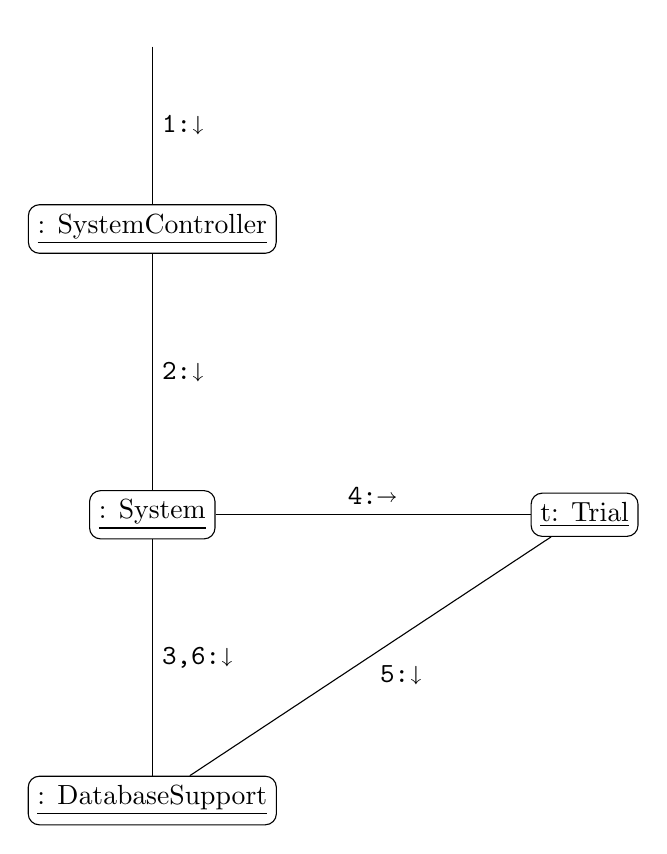
\begin{tikzpicture}[
  auto,
  block/.style = {
    rectangle,
    draw=black,
    align=center,
    rounded corners
  }
]

% Used for the arrow coming down to SystemController
\node[] (start)  {};

%     style     location                variable name    content 
\node[block, below = 2cm of start]      (controller) {\underline{: SystemController}};
\node[block, below = 3cm of controller] (system)     {\underline{: System}}; 
\node[block, right = 4cm of system]     (trial)       {\underline{t: Trial}};
\node[block, below = 3cm of system]     (database)   {\underline{: DatabaseSupport}};

%     (start_node) -- (end_node)   node[location] {content}
\draw (start)      -- (controller) node[midway] {\texttt{1:$\shortdownarrow$}};
\draw (controller) -- (system)     node[midway] {\texttt{2:$\shortdownarrow$}};
\draw (system)     -- (trial)       node[midway] {\texttt{4:$\shortrightarrow$}};
\draw (trial)      -- (database)    node[midway] {\texttt{5:$\shortdownarrow$}};
\draw (system)     -- (database)   node[midway] {\texttt{3,6:$\shortdownarrow$}};

\end{tikzpicture}
\end{center}

\begin{enumerate}
    \item b:=removeJuror(tId: String, jId:String):boolean
    \item b:=removeJuror(tId: String, jId:String):boolean
    \item t:=getTrial(tId: String):Trial
    \item b:=removeJuror(jId: String):boolean
    \item j:=getJuror(jId: String):Juror
    \item b:=putTrial(t:Trial):boolean
    
\end{enumerate}


\end{document}
